%Usepackages
\usepackage{adjustbox, amsmath, amssymb, amsthm, blindtext, bm, bbm, dblfloatfix, esint, fancyhdr, float, graphicx, letltxmacro, marginnote, mathtools, subcaption, xcolor, titlesec, esint}
\usepackage{amssymb}
\usepackage[font={small, it}]{caption}
\usepackage{amsmath}
%\usepackage{floatrow}
\usepackage{times}
\usepackage{ stmaryrd }
\usepackage{amsthm}
\usepackage{xcolor}
\usepackage{mathrsfs}
\usepackage[colorlinks = true,
            linkcolor = black,
            urlcolor  = blue,
            citecolor = black,
            anchorcolor = blue]{hyperref}
% \usepackage[mathscr]{euscript}
\usepackage{mathrsfs}
\usepackage{wasysym}
%\usepackage{pxfonts}
\usepackage[letterpaper, portrait, margin=1in]{geometry}
\usepackage{graphicx}
\usepackage{tikz}
\usepackage{tikz-3dplot}
\usepackage{pgfplots}
\usetikzlibrary{decorations.pathmorphing,patterns}
\usepackage{lipsum}
\usepackage{float}
\usepackage{subcaption}
\usepackage[object=vectorian]{pgfornament}
\usepackage{mwe}
\usepackage{bigints}
\usepackage{titlesec}
\usepackage{halloweenmath}
\setcounter{secnumdepth}{4}
\titleformat{\paragraph}
{\normalfont\normalsize\bfseries}{\theparagraph}{1em}{}
\titlespacing*{\paragraph}
{0pt}{3.25ex plus 1ex minus .2ex}{1.5ex plus .2ex}
\usepackage{mathtools}
\usepackage{pgfplots}
\pgfplotsset{compat=1.15}
\usepackage{lastpage}
\usepackage{enumitem}
\usepackage{tensor}
\usepackage{mathtools}
\usepackage{fancyhdr} 
    \pagestyle{fancy}
    \fancyhf{}
    \rhead{ Page \thepage \  of \pageref{LastPage}}
    \lhead{MATH1410 Final Project}
\usepackage{setspace}
%\usepackage{tikz}
\usetikzlibrary{hobby}

\usepackage{pst-node}

\usepackage{tikz-cd}

% \makeatletter
% \renewcommand\@endtheorem{\vvv@endmarker\endtrivlist\@endpefalse}
% \newcommand\vvv@endmarker{%
%   {\unskip\nobreak\hfil\penalty50
%   \hskip2em\vadjust{}\nobreak\hfil\openbox
%   \parfillskip=0pt \finalhyphendemerits=0 \par
%   \penalty 10000 \parskip=0pt\noindent}\ignorespaces}
% \makeatother

\theoremstyle{definition}

\newtheorem{theorem}{Theorem}[section]
\newtheorem{definition}[theorem]{Definition}
\newtheorem{example}[theorem]{Example}
\newtheorem{lemma}[theorem]{Lemma}
\newtheorem{conjecture}[theorem]{Conjecture}
\newtheorem{exercise}[theorem]{Exercise}
\newtheorem{fact}[theorem]{Fact}
\newtheorem{claim}[theorem]{Claim}
\newtheorem{corollary}[theorem]{Corollary}

\newtheorem{idea}[theorem]{Idea}
\newtheorem{application}[theorem]{Application}
\newtheorem{remark}[theorem]{Remark}

\newtheorem{proposition}[theorem]{Proposition}
\newtheorem{question}[theorem]{Question}
\newenvironment{solution}
  {\renewcommand\qedsymbol{$\blacksquare$}\begin{proof}[Solution]}
  {\end{proof}}
\newenvironment{answer}
  {\begin{proof}[Answer]}
  {\end{proof}}
  
% \newenvironment{example}
%   {\pushQED{\qed}\renewcommand{\qedsymbol}{$\triangle$}\examplex}
%   {\popQED\endexamplex}




%%%%%%%%%%%%%%%%%%%%%%%%%%%%%

%Custom Commands
    \renewcommand\qedsymbol{$\blacksquare$}
    \newcommand{\Pcal}{\mathcal{P}}
    \newcommand{\ve}{\varepsilon}
    \newcommand{\Ocal}{\mathcal{O}}
    \newcommand{\Asf}{\textsf{A}}
    \newcommand{\al}{\alpha}
    \newcommand{\be}{\beta}
    \newcommand{\Nbb}{\mathbb{N}}
    \newcommand{\Si}{\Sigma}
    \newcommand{\Hbb}{\mathbb{H}}
    \DeclareMathOperator{\diag}{diag}
    \newcommand{\De}{\Delta}
    \newcommand{\Xcal}{\mathcal{X}}
    \newcommand{\si}{\sigma}
    \newcommand{\Ga}{\Gamma}
    \newcommand{\Cscr}{\mathscr{C}}
    \newcommand{\1}{\mathbf{1}}
    \newcommand{\Dcal}{\mathcal{D}}
    \newcommand{\Iscr}{\mathscr{I}}
    \newcommand{\Pbb}{\mathbb{P}}
    \newcommand{\B}{\mathbb{B}}
    \newcommand{\Dscr}{\mathscr{D}}
    \newcommand{\Nfrak}{\mathfrak{N}}
    \newcommand{\Efrak}{\mathfrak{E}}
    \DeclareMathOperator{\charp}{charpoly}
    \newcommand{\Csf}{\mathsf{C}}
    \newcommand{\rfrak}{\mathfrak{r}}
    \newcommand{\Sbb}{\mathbb{S}}
    \newcommand{\La}{\Lambda}
    \newcommand{\de}{\delta}
    \DeclareMathOperator{\inte}{int}
    \DeclareMathOperator{\ord}{ord}
    \newcommand{\set}{\mathsf{set}}
    \newcommand{\Bscr}{\mathscr{B}}
    \newcommand{\Zscr}{\mathscr{Z}}
    \newcommand{\ab}{\mathrm{ab}}
    \newcommand{\Xscr}{\mathscr{X}}
    \newcommand{\Escr}{\mathscr{E}}
    \newcommand{\Gscr}{\mathscr{G}}
    \DeclareMathOperator{\Sym}{Sym}
    \newcommand{\om}{\omega}
    \newcommand{\gfrak}{\mathfrak{g}}
    \newcommand{\hfrak}{\mathfrak{h}}
    \newcommand{\kfrak}{\mathfrak{k}}
    \newcommand{\Grp}{\mathsf{Grp}}
    \newcommand{\Ab}{\mathsf{Ab}}
    \newcommand{\xbar}{\bar{x}}
    \newcommand{\abar}{\bar{a}}
    \newcommand{\ybar}{\bar{y}}
    \DeclareMathOperator{\coker}{coker}
    \newcommand{\Modsf}{\mathsf{Mod}}
    \newcommand{\op}{\mathrm{op}}
    \newcommand{\Ring}{\mathsf{Ring}}
    \newcommand{\modsf}{\mathsf{mod}}
    \DeclareMathOperator{\Alt}{Alt}
    \newcommand{\Om}{\Omega}
    \newcommand{\ze}{\zeta}
    \newcommand{\Fcal}{\mathcal{F}}
    \newcommand{\Oscr}{\mathscr{O}}
    \newcommand{\gl}{\mathfrak{gl}}
    \DeclareMathOperator{\Lie}{Lie}
    \DeclareMathOperator{\GL}{GL}
    \DeclareMathOperator{\SL}{SL}
    \DeclareMathOperator{\Vol}{Vol}
    \DeclareMathOperator{\Disc}{Disc}
    \DeclareMathOperator{\SO}{SO}
    \newcommand{\Xfrak}{\mathfrak{X}}
    \DeclareMathOperator{\id}{id}
    \DeclareMathOperator{\Int}{Int}
    \DeclareMathOperator{\End}{End}
    \DeclareMathOperator{\Aut}{Aut}
    \DeclareMathOperator{\stab}{stab}
    \DeclareMathOperator{\orb}{orb}
    \DeclareMathOperator{\grad}{grad}
    \DeclareMathOperator{\curl}{curl}
    \newcommand{\vp}{\varphi}
    \newcommand{\vt}{\vartheta}
    \DeclareMathOperator{\Gal}{Gal}
    \DeclareMathOperator{\rank}{rank}
    \DeclareMathOperator{\col}{col}
    \DeclareMathOperator{\Tame}{Tame}  
    \newcommand{\Yscr}{\mathscr{Y}}
    \newcommand{\Fbb}{\mathbb{F}}
    \newcommand{\Hcal}{\mathcal{H}}
    \newcommand{\arctanh}{\text{arctanh}}
    \newcommand{\pa}{\partial}
    \newcommand{\del}{\boldsymbol{\nabla}}
    \newcommand{\na}{\nabla}
    \newcommand{\Ycal}{\mathcal{Y}}
    \DeclareMathOperator{\spn}{span}
    \DeclareMathOperator{\Inn}{Inn}
    \DeclareMathOperator{\chara}{char}
    \newcommand{\lap}{\nabla^2}
    \newcommand{\Pfrak}{\mathfrak{P}}
    \newcommand{\mfrak}{\mathfrak{m}}
    \newcommand{\Fvec}{\mathbf{F}}
    \newcommand{\Mcal}{\mathcal{M}}
    \newcommand{\ellvec}{\boldsymbol{\ell}}
    \newcommand{\rvec}{\mathbf{r}}
    \DeclareMathOperator{\supp}{supp}
    \newcommand{\Abb}{\mathbb{A}}
    \newcommand{\svec}{\mathbf{s}}
    \newcommand{\VECT}{\mathsf{VECT}}
    \newcommand{\fs}{\vec{\sigma}}
    \newcommand{\bs}{\cev{\sigma}}
    \newcommand{\uvec}{\mathbf{u}}
    \newcommand{\iunit}{\boldsymbol{\hat{\i}}}
    \newcommand{\junit}{\boldsymbol{\hat{\j}}}
    \newcommand{\xunit}{\mathbf{\hat{x}}}
    \newcommand{\Char}{\text{char}}
    \newcommand{\kunit}{\mathbf{\hat{k}}}
    \newcommand{\theunit}{\boldsymbol{\hat{\theta}}}
    \newcommand{\pvec}{\mathbf{p}}
    \newcommand{\qvec}{\mathbf{q}}
    \newcommand{\Qcal}{\mathcal{Q}}
    \newcommand{\yvec}{\mathbf{y}}
    \newcommand{\xvec}{\mathbf{x}}
    \newcommand{\wvec}{\mathbf{w}}
    \newcommand{\bvec}{\mathbf{b}}
    \newcommand{\Ucal}{\mathcal{U}}
    \newcommand{\Ncal}{\mathcal{N}}
    \newcommand{\Scal}{\mathcal{S}}
    \newcommand{\Nscr}{\mathscr{N}}
    \newcommand{\da}{\dagger}
    \newcommand{\CT}{\mathrm{H}}
    \newcommand{\Sscr}{\mathscr{S}}
    \DeclareMathOperator{\lcm}{lcm}
    \newcommand{\evec}{\mathbf{e}}
    \newcommand{\Kscr}{\mathscr{K}}
    \newcommand{\ebold}{\boldsymbol{e}}
    \newcommand{\zvec}{\mathbf{z}}
    \newcommand{\vvec}{\mathbf{v}}
    \newcommand{\Tscr}{\mathscr{T}}
    \newcommand{\avec}{\mathbf{a}}
    \newcommand{\Avec}{\mathbf{A}}
    \newcommand{\Ivec}{\mathbf{I}}
    \newcommand{\ivec}{\mathbf{i}}
    \newcommand{\jvec}{\mathbf{j}}
    \newcommand{\kvec}{\mathbf{k}}
    \newcommand{\of}{\mathfrak{o}}
    \DeclareMathOperator{\Ot}{O}
    \DeclareMathOperator{\Sy}{S}
    \newcommand{\slf}{\mathfrak{sl}}
    \newcommand{\muvec}{\boldsymbol{\mu}}
    \newcommand{\Bvec}{\mathbf{B}}
    \newcommand{\Cvec}{\mathbf{C}}
    \newcommand{\eunit}{\mathbf{\hat{e}}}
    \newcommand{\vpunit}{\boldsymbol{\hat{\varphi}}}
    \newcommand{\zero}{\boldsymbol{0}}
    \newcommand{\tauvec}{\boldsymbol{\tau}}
    \newcommand{\runit}{\mathbf{\hat{r}}}
    \newcommand{\U}{\mathcal{U}}
    \newcommand{\Zbb}{\mathbb{Z}}
    \newcommand{\Bsf}{\mathsf{B}}
    \DeclareMathOperator{\G}{G}
    \newcommand{\gmat}{\textsf{g}}
    \newcommand{\Ccal}{\mathcal{C}}
    \newcommand{\SM}{\mathsf{SM}}
    \newcommand{\VB}{\mathsf{VB}}
    \newcommand{\Dsf}{\mathsf{D}}
    \newcommand{\Fscr}{\mathscr{F}}
    \DeclareMathOperator{\Map}{Map}
    \DeclareMathOperator{\Frob}{Frob}
    \newcommand{\Imat}{\textsf{I}}
    \newcommand{\Rmat}{\textsf{R}}
    \DeclareMathOperator{\Frac}{Frac}
    \DeclareMathOperator{\Spec}{Spec}
    \DeclareMathOperator{\Emb}{Emb}
    \newcommand{\Kcal}{\mathcal{K}}
    \newcommand{\Wcal}{\mathcal{W}}
    \newcommand{\Lcal}{\mathcal{L}}
    \newcommand{\Tcal}{\mathcal{T}}
    \newcommand{\Ecal}{\mathcal{E}}
    \DeclareMathOperator{\im}{im}
    \newcommand{\Qbb}{\mathbb{Q}}
    \newcommand{\ga}{\gamma}
    \newcommand{\la}{\lambda}
    \newcommand{\RomanNumeralCaps}[1]
        {\MakeUppercase{\romannumeral #1}} 
    \newcommand{\dif}{\text{d}}
    \newcommand{\Rbb}{\mathbb{R}}
    \newcommand{\Tbb}{\mathbb{T}}
    \DeclareMathOperator{\Hom}{Hom}
    \DeclareMathOperator{\conv}{conv}
    \newcommand{\Vcat}{\mathsf{V}}
    \newcommand{\Gr}{\text{Gr}}
    \newcommand{\Bcal}{\mathcal{B}}
    \newcommand{\Acal}{\mathcal{A}}
    \newcommand{\pfrak}{\mathfrak{p}}
    \newcommand{\qfrak}{\mathfrak{q}}
    \newcommand{\Evec}{\mathbf{E}}
    \newcommand{\omvec}{\boldsymbol{\omega}}
    \newcommand{\alvec}{\boldsymbol{\alpha}}
    \newcommand{\gvec}{\mathbf{g}}
    \newcommand{\afrak}{\mathfrak{a}}
    \newcommand{\bfrak}{\mathfrak{b}}
    \newcommand{\Cbb}{\mathbb{C}}
    \newcommand{\gavec}{\boldsymbol{\gamma}}
    \newcommand{\Tvec}{\mathbf{T}}
    \newcommand{\Vscr}{\mathscr{V}}
    \newcommand{\Ascr}{\mathscr{A}}
    \newcommand{\Uscr}{\mathscr{U}}
    \newcommand{\Sfrak}{\mathfrak{S}}
    \DeclareMathOperator{\sgn}{sgn}
    \DeclareMathOperator{\vol}{vol}
    \newcommand{\Pscr}{\mathscr{P}}
    \newcommand{\Wscr}{\mathscr{W}}
    \newcommand{\bcdot}{\boldsymbol{\cdot}}
    \DeclareMathOperator{\tr}{tr}
    
    \newcommand{\sectionline}{
        \noindent
        \begin{center}
        {
        {{
        {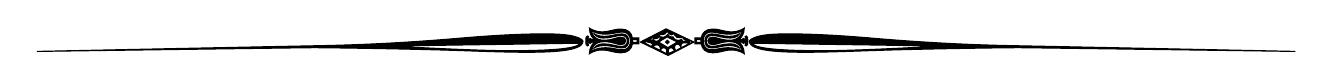
\begin{tikzpicture}
        \node  (C) at (0,0) {};
        \node (D) at (16,0) {};
        \path (C) to [ornament=89] (D);
        \end{tikzpicture}}}}}
        \end{center}
        }
    \newcommand{\sectionlineflip}{
        \noindent
        \begin{center}
        {
        {{
        {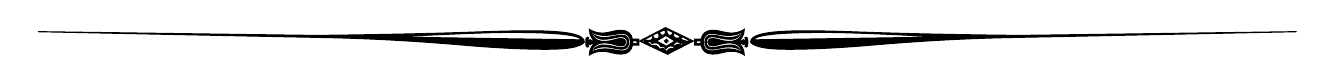
\begin{tikzpicture}
        \node  (C) at (0,0) {};
        \node (D) at (16,0) {};
        \path (D) to [ornament=89] (C);
        \end{tikzpicture}}}}} 
        \end{center}
        }
        

        
       
%%%%%%%%%%%%%%%%%%%%%%%%%%%%%%%
%Custom Symbols
\newcommand{\goodemptyset}[1]{%
\begin{tikzpicture}[#1]%
\draw (0,0) circle (0.1);%
\draw(-0.07,-0.14)--(0.07,0.14);
\end{tikzpicture}%
}

\newcommand{\es}{\raisebox{-1pt}{\goodemptyset{}}}


\makeatletter
\DeclareRobustCommand{\cev}[1]{%
  {\mathpalette\do@cev{#1}}%
}
\newcommand{\do@cev}[2]{%
  \vbox{\offinterlineskip
    \sbox\z@{$\m@th#1 x$}%
    \ialign{##\cr
      \hidewidth\reflectbox{$\m@th#1\vec{}\mkern4mu$}\hidewidth\cr
      \noalign{\kern-\ht\z@}
      $\m@th#1#2$\cr
    }%
  }%
}
\makeatother


\makeatletter
\DeclarePairedDelimiterX{\pmodx}[1]{(}{)}{{\operator@font mod}\mkern6mu#1}
\renewcommand{\pmod}{%
  \allowbreak
  \if@display\mkern18mu\else\mkern8mu\fi
  \pmodx
}
\makeatother
\DeclarePairedDelimiter\bra{\langle}{\rvert}
\DeclarePairedDelimiter\ket{\lvert}{\rangle}
\DeclarePairedDelimiterX\braket[2]{\langle}{\rangle}{#1 \delimsize\vert #2}

 
\makeatletter
\newcommand{\colim@}[2]{%
  \vtop{\m@th\ialign{##\cr
    \hfil$#1\operator@font colim$\hfil\cr
    \noalign{\nointerlineskip\kern1.5\ex@}#2\cr
    \noalign{\nointerlineskip\kern-\ex@}\cr}}%
}
\newcommand{\colim}{%
  \mathop{\mathpalette\colim@{\rightarrowfill@\scriptscriptstyle}}\nmlimits@
}
\renewcommand{\varinjlim}{%
  \mathop{\mathpalette\varlim@{\rightarrowfill@\scriptscriptstyle}}\nmlimits@
}
\renewcommand{\varprojlim}{%
  \mathop{\mathpalette\varlim@{\leftarrowfill@\scriptscriptstyle}}\nmlimits@
}


% %%%%%%%%%%%%%%%%%%%%%%%%%%%%%
% %Just arrows (cause normy arrows suck)
% \newcommand{\goodarrow}[1]{
% \begin{tikzpicture}[#1]
% \draw[-stealth] (0,0)--(0.4,0);
% \end{tikzpicture}
% }

% \renewcommand{\to}{\raisebox{2.4pt}{\hspace{0.08cm}\goodarrow{}\hspace{0.06cm}}}

% %%%%

% \newcommand{\goodtwoheadrightarrow}[1]{
% \begin{tikzpicture}[#1]
% \draw[->>, >=stealth] (0,0)--(0.4,0);
% \end{tikzpicture}
% }

% \renewcommand{\twoheadrightarrow}{\raisebox{2.4pt}{\hspace{0.08cm}\goodtwoheadrightarrow{}\hspace{0.06cm}}}

% %%%

% \newcommand{\goodhookrightarrow}[1]{
% \begin{tikzpicture}[#1]
% \draw[right hook-stealth] (0,0)--(0.4,0);
% \end{tikzpicture}
% }

% \renewcommand{\hookrightarrow}{\raisebox{2.3pt}{\hspace{0.08cm}\goodhookrightarrow{}\hspace{0.06cm}}}

% %%%

% \newcommand{\goodmapsto}[1]{
% \begin{tikzpicture}[#1]
% \draw[-stealth] (0,0)--(0.4,0);
% \draw[] (0,0.06)--(0,-0.06);
% \end{tikzpicture}
% }

% \renewcommand{\mapsto}{\raisebox{0pt}{\hspace{0.02cm}\goodmapsto{}\hspace{0.03cm}}}


% %%%%%%%%%%%%%%%%%%%%%%%%%%%%%

% \tikzcdset{arrow style=tikz, diagrams={>={stealth[round,length=4pt,width=4.5pt,inset=2.75pt]}}}




